\documentclass[../report.tex]{subfiles}

\usepackage{listings}
\usepackage{color}

\definecolor{dkgreen}{rgb}{0,0.6,0}
\definecolor{gray}{rgb}{0.5,0.5,0.5}
\definecolor{mauve}{rgb}{0.58,0,0.82}

\lstset{frame=tb,
  language=Sql,
  aboveskip=3mm,
  belowskip=3mm,
  showstringspaces=false,
  columns=flexible,
  basicstyle={\small\ttfamily},
  numbers=none,
  numberstyle=\tiny\color{gray},
  keywordstyle=\color{blue},
  commentstyle=\color{dkgreen},
  stringstyle=\color{mauve},
  breaklines=true,
  breakatwhitespace=true
  tabsize=3
}

\begin{document}
When designing the data model there were several considerations to make. Our main goals of the data model was as following
\begin{itemize}
\item Make a generic data model that could suit both the ArtShare and SMU Client.
\item Make the model as extendible as possible. By this we mean that we can add a new property to eg a \textit{Media item} without having to change the data model. This facilitates more iterative development.
\item We wanted to have a data model with as high normal form as possible to avoid redundancy in regards to data space and corruption
\end{itemize} 


%Firstly it was important to design a data model which was generic enough to accommodate the demands of the SMU team. Secondly it was important to design a data model which was in as high a normal form as possible in order to reduce redundant data and the possibility of creating corrupt data. Lastly we wanted to make the datamodel as extendible to new features as possible.  


%(WHY DID WE MAKE THE UPLOADER/OWNER OF A MEDIA ITEM A RELATION?!? NOW IT IS POSSIBLE FOR A MEDIA ITEM TO HAVE MORE THAN ONE UPLOADER/OWNER)


Looking at the requirements for \textit{The System} we identified two major entities, namely the \textit{User} and \textit{Media item}. Additionally we realised that we needed an entity representing a \textit{Client} in order for the \textit{ShareIt Back End} to be able to differentiate which \textit{Media Item}s belonged to which \textit{Client}. 

In order to make data model flexible and extendible we choose to only make the \textit{User} and \textit{Media item} store required information. Other information like title, artist, director, email etc. is made relational (The SQL definition of \textit{Media Item} is shown fig \ref{datamodel})

This both facilitates that clients can have different needs to which information is stored on a \textit{User} or \textit{Media item}, but also makes it easier to add more information types iteratively. 

\begin{figure}[H]
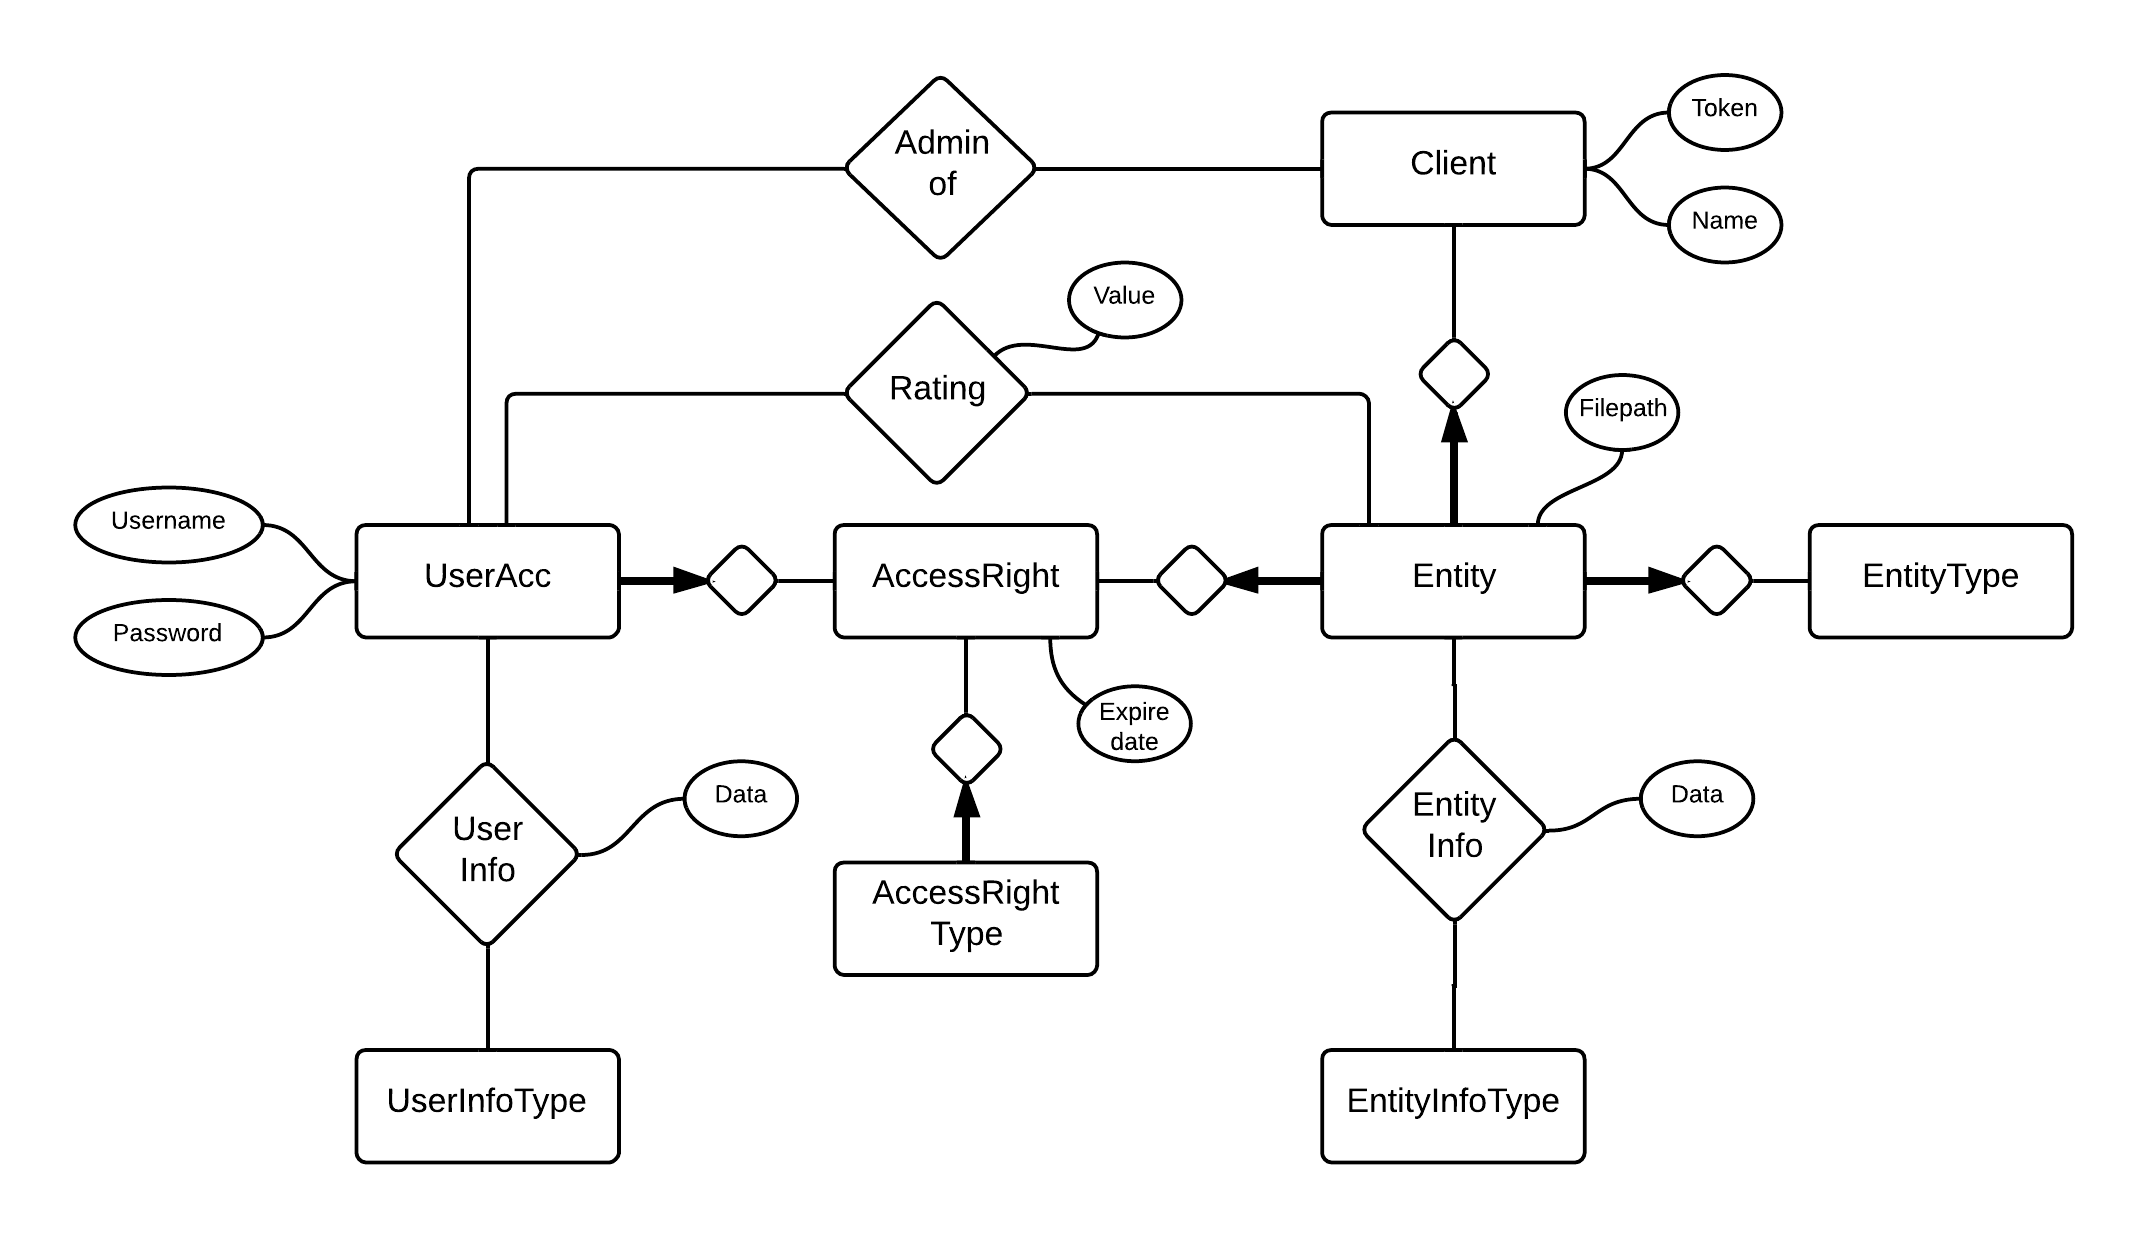
\includegraphics[width=\linewidth]{img/ER.pdf}
\caption{ER diagram of the data model}
\label{fig:use case diagram}
\end{figure}

\begin{figure}[H]
\begin{lstlisting}
CREATE TABLE EntityInfoType(
	Id Int IDENTITY Primary Key,
	Name varchar(256) NOT NULL,
);

CREATE TABLE Entity(
	Id Int IDENTITY Primary Key,
	FilePath varchar(256) NOT NULL,
	ClientId Int NOT NULL REFERENCES Client(Id) ON DELETE CASCADE,
	TypeId Int REFERENCES EntityType(Id)
);

CREATE TABLE EntityInfo(
	Data varchar(max),
	EntityId Int NOT NULL REFERENCES Entity(Id) ON DELETE CASCADE,
	EntityInfoTypeId Int NOT NULL REFERENCES EntityInfoType(Id) ON DELETE CASCADE,
	Id INT IDENTITY Primary Key
);
\end{lstlisting}
\caption{Snippet of Entity (\textit{Media item}) SQL definition}
\label{datamodel}
\end{figure}

Our data model is in 3NF (Third normal form). This is because we have ID's on all entities. An ID for eg \textbf{EntityInfo} (See figure \ref{datamodel} for table definition) is not needed as it could have been a weak entity. We have chosen to give it an ID either way because it was easier to implement a generic Data Access Layer when every entity had an unique property.


\end{document}